%%%%%%%%%%%%%%%%%%%%%%%%%%%%%%%%%%%%%%%%%
% Beamer Presentation
% LaTeX Template
% Version 1.0 (10/11/12)
%
% This template has been downloaded from:
% http://www.LaTeXTemplates.com
%
% License:
% CC BY-NC-SA 3.0 (http://creativecommons.org/licenses/by-nc-sa/3.0/)
%
%%%%%%%%%%%%%%%%%%%%%%%%%%%%%%%%%%%%%%%%%

%----------------------------------------------------------------------------------------
%	PACKAGES AND THEMES
%----------------------------------------------------------------------------------------

\documentclass{beamer}

\mode<presentation> {

% The Beamer class comes with a number of default slide themes
% which change the colors and layouts of slides. Below this is a list
% of all the themes, uncomment each in turn to see what they look like.

%\usetheme{default}
%\usetheme{AnnArbor}
%\usetheme{Antibes}
%\usetheme{Bergen}
%\usetheme{Berkeley}
%\usetheme{Berlin}
%\usetheme{Boadilla}
%\usetheme{CambridgeUS}
%\usetheme{Copenhagen}
%\usetheme{Darmstadt}
%\usetheme{Dresden}
%\usetheme{Frankfurt}
%\usetheme{Goettingen}
%\usetheme{Hannover}
%\usetheme{Ilmenau}
%\usetheme{JuanLesPins}
%\usetheme{Luebeck}
\usetheme{Madrid}
%\usetheme{Malmoe}
%\usetheme{Marburg}
%\usetheme{Montpellier}
%\usetheme{PaloAlto}
%\usetheme{Pittsburgh}
%\usetheme{Rochester}
%\usetheme{Singapore}
%\usetheme{Szeged}
%\usetheme{Warsaw}

% As well as themes, the Beamer class has a number of color themes
% for any slide theme. Uncomment each of these in turn to see how it
% changes the colors of your current slide theme.

%\usecolortheme{albatross}
%\usecolortheme{beaver}
%\usecolortheme{beetle}
%\usecolortheme{crane}
%\usecolortheme{dolphin}
%\usecolortheme{dove}
%\usecolortheme{fly}
%\usecolortheme{lily}
%\usecolortheme{orchid}
%\usecolortheme{rose}
%\usecolortheme{seagull}
%\usecolortheme{seahorse}
%\usecolortheme{whale}
%\usecolortheme{wolverine}

%\setbeamertemplate{footline} % To remove the footer line in all slides uncomment this line
%\setbeamertemplate{footline}[page number] % To replace the footer line in all slides with a simple slide count uncomment this line

%\setbeamertemplate{navigation symbols}{} % To remove the navigation symbols from the bottom of all slides uncomment this line
}

\usepackage{graphicx} % Allows including images
\usepackage{booktabs} % Allows the use of \toprule, \midrule and \bottomrule in tables

%----------------------------------------------------------------------------------------
%	TITLE PAGE
%----------------------------------------------------------------------------------------

\title[Short title]{Matrix Project } % The short title appears at the bottom of every slide, the full title is only on the title page

\author{EE17BTECH11018 \& EE17BTECH11019} % Your name
\institute[IIT Hyderabad] % Your institution as it will appear on the bottom of every slide, may be shorthand to save space
{
IIT Hyderabad \\ % Your institution for the title page
\medskip
\textit{EE 1390-INTRO to AI and ML} 
}
\date{\today} % Date, can be changed to a custom date

\begin{document}

\begin{frame}
\titlepage % Print the title page as the first slide
\end{frame}




\begin{frame}
\frametitle{Geometry Question}
Find a point P on the line 3x+2y+10=0 such that PA+PB is minimum when A is (4,2) and B is (2,4).\\~\\
\end{frame}

\begin{frame}
\frametitle{Figure}
\begin{figure}
\includegraphics[width=0.8\linewidth]{firstpic.png}
\end{figure}
\end{frame}

%------------------------------------------------

\begin{frame}
\frametitle{Matrix Equivalent of Question}
The equation of given line is $ \left[ 
  \begin{array}{ c c }
     3 & 2 
     \end{array} \right]$ x = -10 \newline If we compare this with standard line equation $n{^T}x=c$,we can know that the direction vector of any line normal to this line is n=$ \left[ 
  \begin{array}{ c  }
     3\\
     2
  \end{array} \right]$ and c=-10


\end{frame}

%------------------------------------------------

\begin{frame}
\frametitle{Solution in MATRIX form}
\begin{block}{Idea}
We know A and B are on the same side of the given line. The idea is to take a point A or B and find its image in the given line $A{^\prime}$
\newline We know PA=P$A{^\prime}$.Therefore PA+PB is minimum is same as P$A{^\prime}$+PB is minimum.
\newline $A{^\prime}$ and B are on different sides of the given line and they can form a triangle.Using triangle inequality ,we can say that P$A{^\prime}$+PB is minimum when $A{^\prime}$,P,B are collinear. 
\end{block}

The equation of given line is  $ \left[ 
  \begin{array}{ c c }
     3 & 2 
     \end{array} \right]$ x = -10.\newline Now we find a normal to this line and passing through A=$ \left[ 
  \begin{array}{ c  }
     4\\
     2
  \end{array} \right]$ and let the intersection point be X. The equation of the normal is as following $$ x = A+\lambda(X-A)$$


\end{frame}


\begin{frame}
\frametitle{Solution in MATRIX form}
But we know the direction vector X-A=$ \left[ 
  \begin{array}{ c  }
     3\\
     2
  \end{array} \right]$ .Therefore the equation 

\[
   x =\left[ 
  \begin{array}{ c  }
     4\\
     2
  \end{array} \right ]+ \lambda \left[ 
  \begin{array}{ c  }
     3 \\
     2 
  \end{array} \right]
  \]
 \\  
 \[
  x= \left[ 
  \begin{array}{ c }
     4+3\lambda\\
     2+2\lambda
  \end{array} \right]
  \]
  Since  X lies on normal, Let
\[
 X= 
\left[ 
  \begin{array}{ c  }
     4+3\lambda^{\prime}\\
     2+2\lambda^{\prime}
  \end{array} \right]
  \]
  Now we substitute this point X  in the given line ,we get as follows
  \[
  \left[ 
  \begin{array}{ c c }
     3 & 2
  \end{array}\right] \left[
  \begin{array}{c}
     4+3\lambda^{\prime}\\
     2+2\lambda^{\prime}
     \end{array}\right] = -10
\]     
     
     
  
  
\end{frame}

%---
%------------------------------------------------

\begin{frame}
\frametitle{Solution in MATRIX form}\



 \[3(4+3\lambda^{\prime}+2(2+2\lambda^{\prime}) = -10\]
 \[12+9\lambda^{\prime}+4+4\lambda^{\prime} = -10\]
 \[ 13\lambda^{\prime}=-26\]
 \[\lambda^{\prime}=-2\]
 We know X is midpoint of A and $A^{\prime}$ and $X = A + n \lambda^{\prime}$.Therefore,\\
 
$A^{\prime} = A+ 2n \lambda^{\prime}$  \\ 
\textit{i.e}  $A^{\prime}= \left[ 
  \begin{array}{ c }
     4+3(-2)(2)\\
     2+2(-2)(2)
  \end{array} \right]$
   \end{frame}

%------------------------------------------------

\begin{frame}
\frametitle{Solution in MATRIX form}
A^{\prime}=\left[ 
  \begin{array}{ c }
     -8\\
     -6
  \end{array} \right].
  \newline \text{Now we have to find the line } $A^{\prime}$B which cuts the given line at P (We know that $A^{\prime}$,P,B are on the same line).
 \\The line equation of $A^{\prime}B$ is as follows 
 $$ x = B+ \alpha(A^{\prime}-B)$$
  \[ x= \left[ 
  \begin{array}{ c  }
     2\\
     4
  \end{array} \right]+\alpha(\left[ 
  \begin{array}{ c  }
     -8\\
     -6
  \end{array} \right] - \left[ 
  \begin{array}{ c  }
     2\\
     4
  \end{array} \right])\]
  \[ x= \left[ 
  \begin{array}{ c  }
     2\\
     4
  \end{array} \right]+\alpha(\left[ 
  \begin{array}{ c  }
     -10\\
     -10
  \end{array} \right])
  \]
\end{frame}

\begin{frame}{Solution in MATRIX Form}

\[ x= \left[ 
  \begin{array}{ c  }
     2\\
     4
  \end{array} \right]+\alpha(\left[ 
  \begin{array}{ c  }
     1\\
     1
  \end{array} \right])\]
   Since P lies on the line $A^{\prime}B$  say ,\[ P =\left[ 
  \begin{array}{ c  }
     2+\alpha^{\prime}\\
     4+\alpha^{\prime}
  \end{array} \right]\]
  \\Substituting P in the given line we get,
  \[
  \left[ 
  \begin{array}{ c c }
    3 & 2 \\
     
  \end{array} \right] \left[ 
  \begin{array}{ c  }
     2+\alpha^{\prime}\\
     4+\alpha^{\prime}
  \end{array} \right] =-10
  \]
  \[ 6+3\alpha^{\prime}+8+2\alpha^{\prime}=-10\]
 \end{frame}
\begin{frame}
\frametitle{Solution in MATRIX Form}
\[ 14+ 5\alpha^{\prime} = -10 \]
\[ \alpha^{\prime}= -24/5 \]
\[ P =  \left[ 
  \begin{array}{ c  }
     2-(24/5)\\
     4-(24/5)
  \end{array} \right]\]
  \\Therefore required point P is \[\left[ 
  \begin{array}{ c  }
     -14/5\\
     -4/5
  \end{array} \right] 
  \]
  \\ and the minimum distance PA+PB  is equal to $A^{\prime}B =||B-A^{\prime}||$= $||\left[ 
  \begin{array}{ c  }
     2\\
     4
  \end{array} \right] - \left[ 
  \begin{array}{ c  }
     -8\\
     -6
  \end{array} \right]||$ = $|| \left[ 
  \begin{array}{ c  }
     10\\
     10
  \end{array} \right] ||$ =$10\sqrt{2}$


\end{frame}


\begin{frame}
\frametitle{Figure}
\begin{figure}
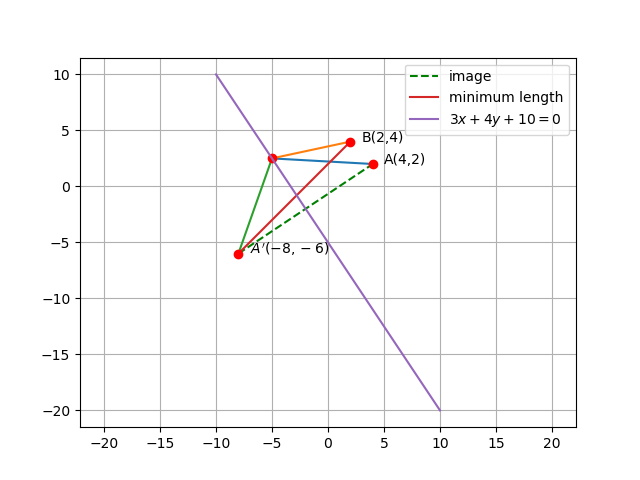
\includegraphics[width=0.8\linewidth]{lastpic.png}
\end{figure}
\end{frame}





\begin{frame}
\Huge{\centerline{The End}}
\end{frame}

%----------------------------------------------------------------------------------------

\end{document}

